\chapter{Can I Completely Change?}

This chapter follows J. Krishnamurti's inquiry into whether human beings can change at the root. The source is the Brockwood Park dialogue from \emph{The Transformation of Man}; the Krishnamurti Foundation Trust source material and LazyingArt LLC curation are credited in the course front matter. No validated frame from this lecture contains a blackboard equation, board diagram, or usable visual notation, so the mathematical structure here is editorial shorthand. We use equations and diagrams only to keep the logic of the spoken inquiry visible.

\section{The Old Question}

The lecture does not begin with a new doctrine. It begins by resuming a question already under pressure: why do human beings live this way? The list is familiar and not abstract: turmoil, confusion, sorrow, conflict, violence, and the misery that continues even when human beings have knowledge, history, religion, politics, therapy, and systems of reform.

The repeated form of the promise is also familiar. Do this and you will be all right. Follow this teacher, this book, this discipline, this political order, this priest, this guru, this analysis. The world has had centuries of such promises, and still the fact remains. Human beings do not live in order, happily, intelligently, without the same chaotic movement continuing.

In compact notation, the failed implication is

\begin{equation}
\mathrm{knowledge}+\mathrm{method}+\mathrm{authority}
\not\Rightarrow
\mathrm{order}.
\end{equation}

This is not a mathematical theorem. It is the opening fact of the lecture. If the usual inputs have not produced order, the next question cannot simply be which method to add. The inquiry asks for the root:

\begin{equation}
Q_0:\qquad
\mathrm{What\ is\ the\ root\ of\ human\ disorder?}
\end{equation}

The rhythm matters. Krishnamurti does not rush from the fact to a conclusion. He lets the question repeat: why? why do we live this way? what is the root? The repetition is part of the discipline. We are not gathering opinions; we are trying to see whether the inquiry reaches the source.

\section{Secondary Explanations}

The first movement tests explanations that are plausible but insufficient. Perhaps sorrow gives a kind of security. Perhaps people get used to conflict and miss it when it is absent. Perhaps war seems to release one from boredom. Perhaps obedience removes the burden of responsibility: the generals decide, and the individual does not have to. Perhaps human beings have become cynical, convinced that human nature cannot be altered.

Each explanation catches something, but the lecture keeps asking whether it reaches the root. The point is not to deny the secondary movements. Habit does operate. Boredom does seek escape. Fear does seek authority. But if we stop there, the inquiry has already become too shallow.

\begin{table}
\centering
\begin{tabular}{p{0.32\linewidth}p{0.56\linewidth}}
\hline
\textbf{Proposed explanation} & \textbf{Why it remains secondary} \\
\hline
Habit & We may become used to conflict, but habit does not explain why conflict is there. \\
False security & Sorrow may feel familiar, but familiarity is not the root of disorder. \\
War as escape & War may interrupt boredom, but the need for escape still has to be understood. \\
Transferred responsibility & Obedience may relieve the burden of choice, but that relief depends on a deeper confusion. \\
Cynicism & The belief that nothing can change may sustain disorder, but it is already part of the disorder. \\
\hline
\end{tabular}
\caption{Secondary explanations matter only when they return the inquiry to the root.}
\end{table}

The working rule is

\begin{equation}
\mathrm{secondary\ explanation}
\neq
\mathrm{root}.
\end{equation}

This is the first mathematical discipline of the chapter. We do not let a partial cause masquerade as the whole structure.

\section{The Planner And The Pattern}

The lecture then turns from humanity in general to the one who is asking. Society may be neurotic, but the observer judging society is not outside society. The movement shifts from ``people'' to ``we,'' and then still more sharply to ``I.'' Why do I not change?

At first the answer seems to lie in fragmentation. Political action, religious action, social action, private pleasure, frustration, belief, and ambition operate as separate movements. They do not form an intelligent whole. They collide with one another, and the person is not outside that collision.

\begin{figure}
\centering
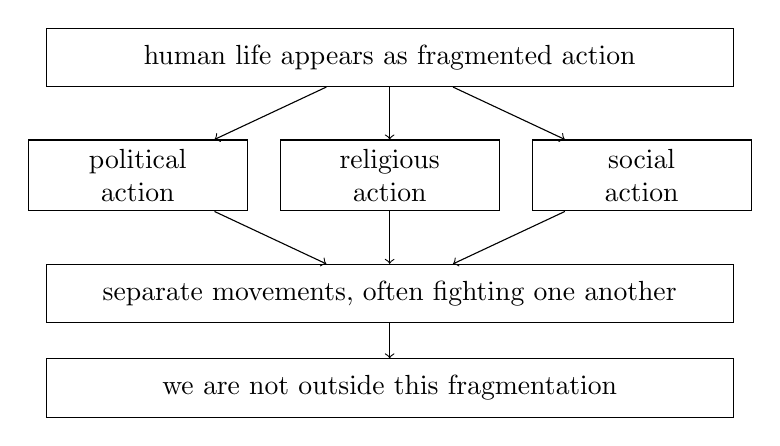
\begin{tikzpicture}[
  box/.style={draw, rectangle, align=center, text width=0.70\linewidth, minimum height=0.74cm},
  smallbox/.style={draw, rectangle, align=center, text width=0.21\linewidth, minimum height=0.72cm}
]
\node[box] (human) at (0,0) {human life appears as fragmented action};
\node[smallbox] (pol) at (-3.2,-1.5) {political\\action};
\node[smallbox] (rel) at (0,-1.5) {religious\\action};
\node[smallbox] (soc) at (3.2,-1.5) {social\\action};
\node[box] (conflict) at (0,-3.0) {separate movements, often fighting one another};
\node[box] (we) at (0,-4.2) {we are not outside this fragmentation};
\draw[->] (human) -- (pol);
\draw[->] (human) -- (rel);
\draw[->] (human) -- (soc);
\draw[->] (pol) -- (conflict);
\draw[->] (rel) -- (conflict);
\draw[->] (soc) -- (conflict);
\draw[->] (conflict) -- (we);
\end{tikzpicture}
\caption{A transcript-backed reconstruction of fragmentation. No screenshot is paired with this figure because no validated visual frame was kept.}
\end{figure}

Let \(D\) denote disorder, \(F\) fragmentation, \(I\) the centre or ``me,'' and \(P\) a projected pattern of change. The lecture's first central structure is this:

\begin{equation}
I_{\mathrm{old}}
\longrightarrow
P_{\mathrm{new}}
\longrightarrow
I_{\mathrm{old}}\ \mathrm{persists}.
\end{equation}

The new pattern may be a book, a discipline, a therapy, a political reorganization, a religious practice, or an image of what I should become. The pattern may look new. The centre that invents and pursues it is old.

\subsection{Question \& Answer}

\paragraph{Question.}
If I want to change, why does change reproduce the old?

\paragraph{Answer.}
Because the entity that wants change designs the pattern of change. The planner remains the same even when the pattern changes. In the dialogue this is restated several times because it is easy to miss: I feel new because I have a new idea, a new system, a new experience. But the ``I'' that adopts the system is the old centre.

A compact version is

\begin{align}
I_{\mathrm{old}} &\longrightarrow P_{\mathrm{new}},\\
P_{\mathrm{new}} &\longrightarrow \mathrm{new\ appearance},\\
I_{\mathrm{old}}+P_{\mathrm{new}} &\not\Rightarrow \mathrm{fundamental\ change}.
\end{align}

\begin{proposition}
A change planned by the old centre is not, by that fact alone, fundamental change.
\end{proposition}

\begin{proof}
The projected change begins with the centre that wants to become something else. That centre forms an image, chooses a method, and pursues an end. Therefore the structure to be transformed is already operating as the author of transformation. The name, colour, vocabulary, or discipline may change, but the source of the movement remains. The result is modification within the old field, not freedom from it.
\end{proof}

This is why the lecture says, in effect, that the old conquers the new. The problem is not merely that self-improvement fails. The sharper point is that the improver may be the very movement that has to be understood.

\section{Authority Created By Disorder}

Once the planner-pattern problem is seen, the lecture rolls it back into a more public and concrete form: authority. Who is my authority? The priest, the analyst, the political leader, the guru, the book, the system, the discipline, the promise that obedience now will bring freedom later?

The inquiry does not merely oppose authority as an attitude. It asks where the demand for authority comes from. The answer is precise: authority arises when I am confused, when I am in disorder. When the field is too chaotic, I assume someone else knows what to do.

Let \(A\) denote authority in this psychological sense: not technical competence, but the inward dependence on another to direct the movement of life. Then

\begin{equation}
D \longrightarrow A.
\end{equation}

But if authority is born from disorder, it cannot end the disorder from which it arises. The loop is

\begin{equation}
D \longrightarrow A \longrightarrow \mathrm{obedience}
\longrightarrow D.
\end{equation}

\begin{figure}
\centering
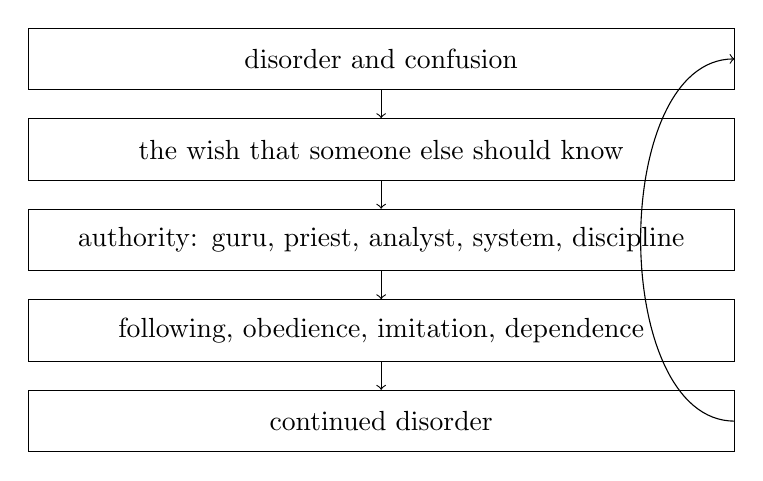
\begin{tikzpicture}[
  box/.style={draw, rectangle, align=center, text width=0.72\linewidth, minimum height=0.78cm}
]
\node[box] (d1) at (0,0) {disorder and confusion};
\node[box] (need) at (0,-1.15) {the wish that someone else should know};
\node[box] (auth) at (0,-2.30) {authority: guru, priest, analyst, system, discipline};
\node[box] (follow) at (0,-3.45) {following, obedience, imitation, dependence};
\node[box] (d2) at (0,-4.60) {continued disorder};
\draw[->] (d1) -- (need);
\draw[->] (need) -- (auth);
\draw[->] (auth) -- (follow);
\draw[->] (follow) -- (d2);
\draw[->] (d2.east) .. controls (2.9,-4.6) and (2.9,0) .. (d1.east);
\end{tikzpicture}
\caption{The authority loop: disorder creates the appeal of authority, and dependence sustains disorder.}
\end{figure}

The point is not a crude attack on teachers or doctors. It is a structural claim. If my appeal to authority springs from confusion, then the appeal carries the confusion forward.

\subsection{Question \& Answer}

\paragraph{Question.}
Must I follow authority in order to see my dependence on authority?

\paragraph{Answer.}
The lecture refuses that thesis. To follow authority in order to discover the danger of following authority is already to continue dependence. The same logic appears in the discussion of self-deception: must I deceive myself in order to understand self-deception? If the deception is genuine, the mind does not know what it is doing.

The rejected implications are

\begin{align}
\mathrm{following\ authority}
&\not\Rightarrow
\mathrm{freedom\ from\ authority},\\
\mathrm{self\mbox{-}deception}
&\not\Rightarrow
\mathrm{understanding\ of\ self\mbox{-}deception}.
\end{align}

This local question preserves an important tension in the lecture. The speakers are not making a slogan against therapy, politics, or religion. They are testing a proposed route: dependence used as the path out of dependence. The route fails because it reproduces the structure it claims to dissolve.

\section{Correct Action Without A Guide}

The sane rejection of authority is the next transition. It is not rebellion, bitterness, or a decorative independence. It is sane because the source of authority has been seen. Disorder created it; therefore psychological dependence on it cannot end disorder.

Now the question becomes practical. If no authority can tell me, what is correct action? How shall I live? Who will answer: Marx, Lenin, Mao, the Pope, the priest, the analyst, the guru? The lecture does not replace one authority with another. It changes the question.

\begin{align}
Q_1 &: \quad \mathrm{What\ is\ correct\ action?}\\
Q_2 &: \quad \mathrm{Can\ the\ mind\ be\ free\ of\ disorder?}
\end{align}

The second question is prior because action is not independent of the mind that acts. A confused mind cannot discover correct action by formula. Nor can it receive correct action as an instruction from another confused mind.

A cautious compression is

\begin{equation}
\mathrm{correct\ action}
\quad \mathrm{requires} \quad
\mathrm{absence\ of\ inward\ disorder}.
\end{equation}

This should not be read as a moral law. It is an observational necessity. If the actor is fragmented, ambitious, frightened, or dependent, then action carries that fragmentation, however noble its language.

\paragraph{A worked reduction.}
The lecture's move can be set out in steps:

\begin{enumerate}
\item I ask, ``What is the right action?''
\item If I am confused, my answer is shaped by confusion.
\item If I ask an authority out of confusion, the asking continues the same movement.
\item Therefore the first task is not to obtain instruction.
\item The first task is to see whether the mind can understand and be free of its disorder.
\end{enumerate}

This produces energy rather than escape. The mind is no longer handing responsibility to teachers, systems, holy places, analysts, or promises. It is not looking for another pattern. The seriousness gathers because the question is now one's life.

The lecture also makes a fine distinction here. We may meet as friends and investigate, but that is not cooperation in the ordinary sense if both minds are confused. Cooperation may become collusion in disorder. The safer word is investigation: not one mind leading another, but a direct looking into what is.

\section{The Word, The Thing, And Psychological Reality}

The inquiry now asks what disorder is made of. Krishnamurti limits the word consciousness for the moment. In this restricted use, consciousness is the accumulated movement of fragments: beliefs, memories, conclusions, images, words, desires, fears, and thought. The qualification matters. This is not a complete theory of consciousness. It is the field under examination in this dialogue.

Let \(C\) denote consciousness in that limited sense. Then

\begin{equation}
C \approx
\mathrm{beliefs}
+\mathrm{memories}
+\mathrm{conclusions}
+\mathrm{images}
+\mathrm{fragmented\ thought}.
\end{equation}

The ``me'' is not outside this collection. The me is made by it, and it separates:

\begin{equation}
\mathrm{me}
\longrightarrow
\mathrm{separation}
\longrightarrow
D.
\end{equation}

Here the lecture encounters a language problem. If I am the movement I am trying to observe, how can I look at it? If the words are made by the very system under investigation, how can words help? The answer is not to abandon language, but to use it carefully. The word is not the thing.

\begin{equation}
\mathrm{word} \neq \mathrm{thing}.
\end{equation}

The word is thought. A belief is thought. A conclusion is thought. But a belief may feel intensely real. To the believer, God, nation, ideology, self, or theory is not merely a word. It is reality.

We can track the movement as

\begin{align}
\mathrm{word} &\in \mathrm{thought},\\
\mathrm{thought} &\longrightarrow \mathrm{image\ or\ belief},\\
\mathrm{belief} &\longrightarrow R_{\mathrm{psychological}}.
\end{align}

\begin{definition}
\(R_{\mathrm{psychological}}\) denotes the felt reality produced or sustained by belief, image, word, conclusion, or self-sense. It may be illusory, but it has compelling force for the mind that believes it.
\end{definition}

The lecture is careful about nature. Thought did not create nature. Thought can describe nature, measure it, write poetry about it, and make theories about it. But thought has also put together chairs, tables, machines, social structures, beliefs, and illusions. Inwardly, the illusion it creates may function as reality.

This distinction prevents the chapter from drifting into imported metaphysics. The point is local and exact: investigation stops when belief is treated as fact. If I say, ``This belief is reality,'' the door closes. The living question is whether the mind can see belief as belief and watch the movement by which the word becomes the thing.

\section{Can Thought Be Aware Of Itself?}

The final movement gathers the earlier steps. Authority has been rejected because it arises from disorder. Correct action cannot be supplied from outside. The me is disorder because it divides. Consciousness, for the purpose of this inquiry, is the accumulated movement of fragments. Words and beliefs become psychological realities. Now the question becomes sharper:

\begin{equation}
Q_3:\qquad
\mathrm{Can\ consciousness\ be\ aware\ of\ itself?}
\end{equation}

Or, more simply, with \(T\) denoting thought as movement,

\begin{equation}
T \overset{?}{\longrightarrow} \mathrm{awareness\ of\ }T.
\end{equation}

This is not thought as a fixed object. It is thought moving: making images, forming beliefs, dividing me from you, constructing psychological reality, and asking how to escape the disorder it has produced.

\subsection{Question \& Answer}

\paragraph{Question.}
Can thought be aware of its own movement, and does that awareness alter the movement?

\paragraph{Answer.}
The lecture does not answer by giving a method. It asks that the question be tested directly: can thought be aware of itself, of its structure, activity, nature, and consequences? Can the doer be aware of the doing?

A cautious notation is

\begin{equation}
\mathrm{awareness}\!\left(T_{\mathrm{movement}}\right)
\overset{?}{\longrightarrow}
\mathrm{radical\ change}.
\end{equation}

The uncertainty mark is essential. The dialogue briefly says that thought ``stops,'' but then refines the statement: it is undergoing a radical change. We should not turn ``stops'' into a doctrine. The lecture is pointing to the possibility that direct observation changes the movement observed.

A physical analogy is mentioned near the end: in observation, the object may not be fixed apart from the act of observation. The chapter should not turn that remark into quantum theory. It is an analogy, not a derivation. The inward question remains: what takes place when thought is aware of its own movement?

\begin{figure}
\centering
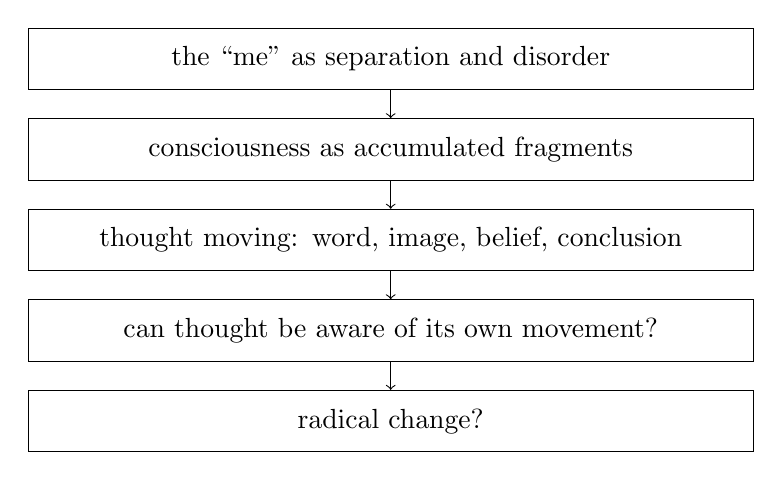
\begin{tikzpicture}[
  box/.style={draw, rectangle, align=center, text width=0.74\linewidth, minimum height=0.78cm}
]
\node[box] (me) at (0,0) {the ``me'' as separation and disorder};
\node[box] (c) at (0,-1.15) {consciousness as accumulated fragments};
\node[box] (t) at (0,-2.30) {thought moving: word, image, belief, conclusion};
\node[box] (aware) at (0,-3.45) {can thought be aware of its own movement?};
\node[box] (change) at (0,-4.60) {radical change?};
\draw[->] (me) -- (c);
\draw[->] (c) -- (t);
\draw[->] (t) -- (aware);
\draw[->] (aware) -- (change);
\end{tikzpicture}
\caption{The final inquiry remains open. Awareness of thought's movement is not presented as a technique or guaranteed result.}
\end{figure}

The lecture ends by saving the next question for another conversation: time. That restraint is part of the ending. We do not close the inquiry with a formula. We leave it where the dialogue leaves it, with the question active.

\section{Summary}

The lecture moves from the public fact of human disorder to the intimate question of whether change at the root is possible. It tests secondary explanations--habit, false security, war as escape, surrendered responsibility, cynicism--but does not let any of them replace the root inquiry.

The central mathematical structure is simple and severe:

\begin{equation}
I_{\mathrm{old}}
\longrightarrow
P_{\mathrm{new}}
\longrightarrow
I_{\mathrm{old}}\ \mathrm{continues}.
\end{equation}

The one who wants to change may be part of the disorder. The planner creates new patterns while remaining the old centre. The same structure appears as authority:

\begin{equation}
D \longrightarrow A \longrightarrow D.
\end{equation}

Disorder creates the demand for someone else to know, and dependence sustains the disorder.

From there the inquiry turns to correct action, consciousness, language, belief, and psychological reality. The word is not the thing, yet belief can make the word feel real. The me is not outside this movement; it is made of it and divides through it.

The final question is left deliberately unfinished:

\begin{equation}
\mathrm{Can\ thought\ be\ aware\ of\ its\ own\ movement?}
\end{equation}

The chapter should preserve that ending. It is not a method, not a promise, and not a conclusion. It is the point at which the inquiry becomes exact enough to continue.